% !TEX root = tracking.tex
\section{Introduction}
Many applications of autonomous dynamical systems will require the ability to plan trajectories in real time while maintaining safety.  
% As unmanned aerial vehicles (UAVs) and other autonomous systems become more commonplace, it is essential that they be able to plan safe motion paths through crowded environments in real-time. 
This is particularly crucial for navigating through environments that are \textit{a priori} unknown, because re-planning based on updated information about the environment is often necessary. 
Achieving safe navigation in real time is difficult for many common dynamical systems due to computational complexity.
 In order to achieve real-time planning, many algorithms use highly simplified model dynamics or kinematics.  The resulting plans may not be dynamically feasible for the true autonomous system, resulting in a tracking error between the planned path and the executed trajectory.
 This concept is illustrated in Fig. \ref{fig:chasing}, where the path was planned using a simplified planning model, but the real vehicle cannot track this path exactly. 
External disturbances (e.g. wind) can be difficult to account for using real-time path or trajectory planning algorithms, causing an additional source of tracking error. 
These tracking errors can lead to dangerous situations in which the planned path is safe, but the actual system trajectory enters unsafe regions.
 
 %Real-time planning that is both safe and accurate presents a very difficult challenge: accuracy and robustness in many dyanimcal systme sis difficult to compute, often precluding real-time computer hands.fast planning is generally at odds with the need for maintaining safety and robustness.  

We propose the modular tool FaSTrack: Fast and Safe Tracking, which models the navigation task as a sophisticated \textit{tracking system} that pursues a simplified \textit{planning system}. 
The tracking system accounts for complex system dynamics as well as bounded external disturbances, while the simple planning system enables the use of real-time planning algorithms. 
Offline, a precomputed pursuit-evasion game between the two systems can be analyzed using any suitable method. 
This results in a \textit{tracking error function} that maps the initial relative state between the two systems to the \textit{tracking error bound} (TEB): the maximum possible relative distance that could occur over time. 
This TEB can be thought of as a ``safety bubble" around the planning system that the tracking system is guaranteed to stay within. 
Because the tracking error is bounded in the relative state space, we can precompute and store a \textit{safety control function} that  maps the real-time relative state to the optimal safety control for the tracking system to ``catch" the planning system. 
The offline computations are \textit{independent} of the path planned in real-time.

Online, the autonomous system senses obstacles, which are then augmented by the TEB to ensure that no potentially unsafe paths can be computed. 
Next, a path or trajectory planner uses the simplified planning model to determine the next desired state. 
The tracking system then finds the relative state between itself and the next desired state. 
If this relative state is nearing the TEB then it is plugged into the safety control function to find the instantaneous optimal safety control of the tracking system; otherwise, any controller may be used. In this sense, FaSTrack provides a \emph{least-restrictive} control law. 
This process is repeated as long as desired. 
  
\begin{figure}
	\centering
	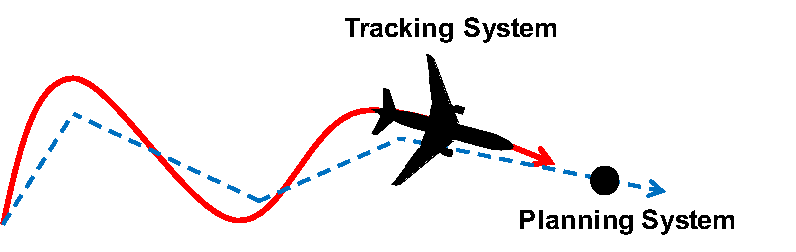
\includegraphics[width=0.35\textwidth]{fig/chasing}
	\caption{Left: A planning system (blue disk) using a fast but simple model, followed by a tracking system (green plane) using a more complex model, navigating through an environment with obstacles. By using FaSTrack the tracking system is guaranteed to stay within some TEB (blue circle). Right: Safety and goal-satisfaction can be guaranteed by planning with respect to obstacles augmented by the TEB (large blue circles).}
	\label{fig:chasing}
\end{figure}
%

FaSTrack was designed to be modular, and can be used with any method for computing the TEB in conjunction with any existing fast path or trajectory planning algorithms.  
This enables motion planning that is real-time, guaranteed safe, and dynamically accurate. 
In this paper, we demonstrate the FaSTrack framework by using three different real-time planning algorithms that have been ``robustified" by precomputing the TEB and safety control function. 
The planning algorithms used in our numerical examples are the fast sweeping method (FSM) \cite{Takei2013}, rapidly-exploring random trees (RRT) \cite{Kuffner2000,Kavraki1996}, and model-predictive control (MPC) \cite{Qin2003}. 
In the three examples, we also consider different models for the tracking system and the planning system.
The precomputation of the TEB and safety control function for each planning-tracking system pair is done by solving a Hamilton-Jacobi (HJ) partial differential equation (PDE). 
In the simulations, the system travels through a static environment with constraints defined, for example, by obstacles, while experiencing disturbances.
The constraints are only fully known through online sensing, for example, once obstacles are within the limited sensing region of the vehicle. 
By combining the TEB with real-time planners, the system is able to safely plan and track a trajectory through the environment in real time. 
